\documentclass[notes,color]{sepslide0}
\usepackage{graphicx}
\usepackage[overheads]{mysepslides}
\usepackage{tech,graphicx,url,tikz,scalalistings}

\title{Clients and Servers} 
\author{Gavin Lowe}

% \everymath{\color{Plum}}
% \def\smaller{\small} 
\def\scalacolour{\color{violet}}

\begin{document}

\begin{slide}
  
  \Title

Reading: Andrews, Section 7.3.

\end{slide}

%%%%%


\begin{slide}
\heading{Clients and servers}

A common pattern in concurrent systems is that of clients and servers.  A
\emph{server} is a thread or process that repeatedly handles requests from
\emph{client}s.
%
\begin{itemize}
\item Many modules, such as concurrent datatypes, can be easily implemented in
this way.

\item This is a pattern that is often used in the implementation of operating
systems.

\item It's the pattern that is prevalent in networked systems.
\end{itemize}
\end{slide}

%%%%%

\begin{slide}
\heading{Example: a resource server}

Consider a server that is responsible for managing and allocating multiple
resources of the same kind, such as memory or file blocks.  Clients acquire
resources for use, and later return them to the server.

What should happen if a client requests a resource and there is none
available?  We choose to use an |Option[Resource]| value:
%
\begin{itemize}
\item A value |Some(r)| indicates that resource |r| has been acquired;

\item The value |None| indicates that no resource was available.
\end{itemize}
%
In the latter case, it is up to the client to decide what to do (maybe try
again later, or maybe throw an exception).

An alternative would be for the server to queue the request until it can be
serviced. 
\end{slide}

%%%%%

\begin{slide}
\heading{Example: a resource server}

We will define a server with the following interface. 
%
\begin{scala}
/** A resource server. */
trait RAServer{
  /** Client identities. */
  type ClientId = Int

  /** Resource identities. */
  type Resource = Int

  /** Request a resource. */
  def requestResource(me: ClientId): Option[Resource]

  /** Return a resource. */
  def returnResource(me: ClientId, r: Resource) 
} 
\end{scala}
\end{slide}

%%%%%

\begin{slide}
\heading{First implementation}

In the first implementation, we assume clients have identities in the range
|[0..clients)|, and resources have identities in the range
  |[0..numResources)|, with |clients| and |numResources| known in advance.
%
\begin{scala}
/** A resource server. 
  * This version assumes the number of clients is known initially. 
  * @param clients the number of clients.
  * @param numResources the number of resources.  */
class RAServer1(clients: Int, numResources: Int) extends RAServer{
  ...
}
\end{scala}
\end{slide}

%%%%%

\begin{slide}
\heading{Channels}

Internally, clients will send requests to a server thread, and receive replies
back. 
%
We use one channel per client to allow the server to allocate resources.  We
use two buffered channels to allow clients to request or return resources.
%
\begin{scala}
class RAServer1(clients: Int, numResources: Int) extends RAServer{
  /* Channel for requesting a resource. */
  private val acquireRequestChan = new BuffChan[ClientId](clients)

  /* Channels for optionally allocating a resource, indexed by client IDs. */
  private val acquireReplyChan = 
    Array.fill(clients)(new BuffChan[Option[Resource]](1))

  /* Channel for returning a resource. */
  private val returnChan = new BuffChan[Resource](clients)
  ...
}
\end{scala}
\end{slide}

%%%%%

\begin{slide}
\heading{Client operations}

\begin{scala}
  /** Request a resource. */
  def requestResource(me: ClientId): Option[Resource] = {
    acquireRequestChan!me  // send request
    acquireReplyChan(me)?() // wait for response
  }

  /** Return a resource. */
  def returnResource(me: ClientId, r: Resource) = returnChan!r
\end{scala}
\end{slide}


%%%%%

\begin{slide}
\heading{The server}

The server needs to keep track of the resources that are currently free; we
use an array \SCALA{free} for this:
%
\begin{scala}
  private def server = thread{
    // Record whether resource i is available in free(i)
    val free = Array.fill(numResources)(true)

    serve( 
      ...
    )
  }

  // Fork off the server
  server.fork
\end{scala}
%
Note that only the server has access to |free|, which avoids race
conditions.  Declaring variables inside a server can clarify their scope. 
\end{slide}

%%%%%

\begin{slide}
\heading{The server main loop}

\begin{scala}
    serve(
      acquireRequestChan =?=> { c => 
	// Find free resource
	var r = 0
	while(r < numResources && !free(r)) r += 1
	if(r == numResources) acquireReplyChan(c)!None
        else{  // Pass resource r back to client c
	  free(r) = false; acquireReplyChan(c)!Some(r)
        }
      }
      | returnChan =?=> { r => free(r) = true }
    )
\end{scala}
\end{slide}




%%%%%

\begin{slide}
\heading{Shutting down the server}

It might be necessary to shut down the server, allowing the server thread to
terminate. 
%
\begin{scala}
  /* Channel for shutting down the server. */
  private val shutdownChan = new SyncChan[Unit]

  /** Shut down the server. */
  def shutdown = shutdownChan!()
  
  private def server = thread{
    ...
    serve(
      acquireRequestChan =?=> { c => ... }
      | returnChan =?=> { r => ... }
      | shutdownChan =?=> { _ =>
          acquireRequestChan.close; returnChan.close; shutdownChan.close }
    )
  }
\end{scala}  
\end{slide}
 % intro, resource allocation example

\begin{slide}
\heading{Testing}

How can we test the resource server?  

The property we want to test is that two clients never hold the same resource:
if a resource~$r$ is allocated to client~$c_1$, it can't be allocated to
another client~$c_2$ until $c_1$ has returned it.

Idea: run a number of clients, who randomly request and return resources; log
these actions; test whether the resulting trace of log events is valid.
\end{slide}

%%%%%

\begin{slide}
\heading{Logging}

We use a log of type |Log[LogEvent]| where
\begin{scala}
  // Events put into the log
  trait LogEvent
  case class GotResource(c: ClientId, r: Resource) extends LogEvent
  case class ReturnedResource(c: ClientId, r: Resource) extends LogEvent
\end{scala}

Subsequently, we can use the |get| method on the log, to get the
results of logging as an |Array[LogEvent]|.  
\end{slide}

%%%%%

\begin{slide}
\heading{A client for testing}

\begin{scala}
  def client(me: ClientId, resourceServer: RAServer, log: Log[LogEvent]) = thread{
    var got = new scala.collection.mutable.Queue[Resource]() // resources held
    for(_ <- 0 until iters){
      if(Random.nextInt(2) == 0){        // Acquire new resource
	resourceServer.requestResource(me) match{
          case Some(r) =>  log.add(me, GotResource(me, r)); got.enqueue(r)
          case None => {}  // try again
        }
      }
      else if(got.nonEmpty){    	// Return resource
	val r = got.dequeue
        log.add(me, ReturnedResource(me, r))
	resourceServer.returnResource(me, r)
      }
    }
  }
\end{scala}
\end{slide}  

%%%%%

\begin{slide}
\heading{Logging}

Note that we log acquiring resources \emph{after} the resource is acquired,
and log returning resources \emph{before} the resource is returned.  This
means that the period during which the log indicates that the thread holds a
resource is a \emph{subset} of the true time.

This is necessary to avoid false positives (the testing signalling an error,
when in fact there is none).  If we were to return a resource before logging
the return, it is possible that a client would be slow in logging the return,
and that another client might have obtained the same resource in the mean
time, giving a false positive.

However, this does risk false negatives (the testing failing to detect an
incorrect behaviour).  But if there is a bug, doing enough testing should also
produce true positives. 
\end{slide}

%%%%%

\begin{slide}
\heading{Running a test}

\begin{scala}
  /** Run a single test. */
  def runTest = {
    val log = new Log[LogEvent](p)
    val resourceServer = new RAServer(p, numResources)
    run(||(for (i <- 0 until p) yield client(i, resourceServer, log)))
    resourceServer.shutdown
    if(!checkLog(log.get)) sys.exit
  }
\end{scala}

The |main| function calls |runTest| many times. 
\end{slide}

%%%%%

\begin{slide}
\begin{scala}
  /** Check that events represents a valid log: if a GotResource event happens,
    * no thread is currently holding the resource. */
  def checkLog(events: Array[LogEvent]): Boolean = {
    val held = Array.fill(numResources)(false)  // Which resources are held
    var error = false; var i = 0
    while(i < events.size && !error){
      events(i) match{
        case GotResource(c, r) =>
          if(held(r)){ // error!
            println("Error found:"); println(events.take(i+1).mkString("\n"))
            error = true
          }
          else held(r) = true
        case ReturnedResource(c, r) => held(r) = false
      }
      i += 1
    }
    !error
  }
\end{scala}
\end{slide}

%%%%%%%%%%%%%%%%%%%%%%%%%%%%%%%%%%%%%%%%%%%%%%%%%%%%%%% 

\begin{slide}
\heading{Arbitrary many clients}

So far, we have assumed a fixed number of clients, with this number known when
the resource server is created.  This allowed us to create one reply channel
per client.

If we do not know the number of clients, an alternative is for each client to
create a new reply channel for each request, and to send the reply channel
within the request.  The server can then reply on this reply channel.  

We illustrate this technique in the following slides (omitting the parts that
are unchanged). 
\end{slide}

%%%%%

\begin{slide}
\heading{Requesting resources}

\begin{scala}
  private type ReplyChan = Chan[Option[Resource]]
  /* Channel for requesting a resource. */
  private val acquireRequestChan = new BuffChan[ReplyChan](clients)

  /** Request a resource. */
  def requestResource(me: ClientId): Option[Resource] = {
    val replyChan = new BuffChan[Option[Resource]](1)
    acquireRequestChan!replyChan  // send request
    replyChan?() // wait for response
  }
\end{scala}
\end{slide}

%%%%%

\begin{slide}
\heading{The server}

\begin{scala}
  private def server = thread{
    ...
    serve(
      acquireRequestChan =?=> { replyChan => 
	// Find free resource
	var r = 0
	while(r < numResources && !free(r)) r += 1
	if(r == numResources) replyChan!None
        else{  // Pass resource r back to client 
	  free(r) = false; replyChan!Some(r)
        }
      }
      | ...
    )
  }
\end{scala}
\end{slide}

%%%%%%%%%%%%%%%%%%%%%%%%%%%%%%%%%%%%%%%%%%%%%%%%%%%%%%%

\begin{slide}
\heading{Storing requests}

Previously, if the server couldn't meet a request, it immediately replied with
a |None| value.  

An alternative would be to queue such requests until they can be met.

Note that this can lead to a deadlock if all resources are allocated, and all
clients are requesting more.
\end{slide}

%%%%%

\begin{slide}
\heading{The server}

The server keeps track of the pending requests in a queue.
%
\begin{scala}
  private def server = thread{
    // Record whether resource i is available in free(i)
    val free = Array.fill(numResources)(true)
    // Reply channels for requests that cannot be served immediately.
    val pending = new scala.collection.mutable.Queue[ReplyChan]
    // Invariant: if pending is non-empty, then all entries in free are false.

    serve(
      ...
    )
  }
\end{scala}
\end{slide}

%%%%%

\begin{slide}
\heading{The server}

\begin{scala}
    serve(
      acquireRequestChan =?=> { replyChan => 
	// Find free resource
	var r = 0
	while(r < numResources && !free(r)) r += 1
	if(r == numResources) pending.enqueue(replyChan) // client has to wait
        else{  // Pass resource r back to client 
	  assert(pending.isEmpty); free(r) = false; replyChan!Some(r)
        }
      }
      | returnChan =?=> { r =>
          if(pending.nonEmpty)
            pending.dequeue!Some(r) // allocate r to blocked client
          else free(r) = true
      }
      | shutdownChan =?=> { _ => ... }
    )
\end{scala}
\end{slide}

%%%%%

\begin{slide}
\heading{Blocking unsatisfiable requests}

Here's a simpler way to achieve the same effect.  Rather than the server
explicitly queueing pending requests, the clients can be blocked on the
|acquireRequestChan| channel until there is a resource free.

\end{slide}

%%%%%

\begin{slide}
\heading{Blocking unsatisfiable requests}

\begin{scala}
  private def server = thread{
    // Record whether resource i is available in free(i)
    val free = Array.fill(numResources)(true)
    // The number of free resources, equal to the number of trues in free.
    var numFree = numResources

    serve(
      numFree > 0 && acquireRequestChan =?=> { replyChan => 
	var r = 0; while(r < numResources && !free(r)) r += 1
	assert(r < numResources); free(r) = false; numFree -= 1
        replyChan!Some(r)
      }
      | returnChan =?=> { r => free(r) = true; numFree += 1 }
      | shutdownChan =?=> { ... } // as before
    )
  }
\end{scala}
\end{slide}

%%%%%

\begin{slide}
\heading{Blocking unsatisfiable requests}

Note that when the server has no free resources, all client threads wanting to
obtain a resource will be blocked on |acquireRequestChan|.

When a resource is returned, those clients will compete to communicate on the
channel.  The one that wins will obtain the resource.

This means that this version is probably less fair than the previous one.
Whether this is important depends on the use case.
\end{slide}

%%%%%%%%%%%%%%%%%%%%%%%%%%%%%%%%%%%%%%%%%%%%%%%%%%%%%%%


\begin{slide}
\heading{Introducing asynchrony}

At present, the client sends a request, and then stops and waits for a
response: this is rather like a procedure call.

In some cases, the client could do some useful work while waiting for the
request to be serviced:
%
\begin{scala}
<make request>
<other useful work>
<obtain response>
\end{scala}
%

We could change the interface of the object to support this, decoupling the
request for a resource from obtaining the resource.

The fact that we have used buffered reply channels means that the server can
send the response even if the client isn't yet ready for it.  


%% (This would change the interface of the corresponding object.)

%% What happens if the server is ready to return the response before the client
%% is ready to receive it?
\end{slide}

%% %%%%%

%% \begin{slide}
%% \heading{Using buffering}

%% CSO includes buffered communication channels.  

%% A sender can add values to a buffered channel, up to the capacity of the
%% channel, without waiting for a receiver to be ready.

%% Buffered channels should be used when there is no need for the
%% processes to synchronise.

%% |OneOneBuf[T](size)| returns a (one-one) buffered channel of type \SCALA{T}
%% that can hold up to \SCALA{size} messages.

%% |N2NBuf[T](size, writers, readers)| returns a buffered channel of type \SCALA{T}
%% that can hold up to \SCALA{size} messages, to be used by |writers| writers and
%% |readers| readers.

%% \end{slide}

%% %%%%%

%% \begin{slide}
%% \heading{Using buffering}

%% It makes sense to make the channels from the clients to the server buffered,
%% to reduce the likelihood of the clients having to wait for the
%% server; we give them capacity \SCALA{clients}.
%% \begin{scala}
%%   private val acquireRequestChan = 
%%     N2NBuf[ReplyChan](size = clients, readers = 1, writers = clients)
%%   private val returnChan = 
%%     N2NBuf[Resource](size = clients, readers = 1, writers = clients)
%% \end{scala}

%% It also makes sense to make the response channels buffered, so the server does
%% not have to wait for a client; they only need have capacity~1.
%% %
%% \begin{scala}
%%   val replyChan = OneOneBuf[Option[Resource]](size = 1)
%% \end{scala}
%% \end{slide}

%%%%%

\begin{slide}
\heading{Multiple request channels versus multiple request types}

We chose to use different channels for different requests to the server.  An
alternative is to use a single channel, and multiple types of request.

Such an approach seems more natural in a networked application.
\end{slide}

%%%%%


\begin{slide}
\heading{Multiple request channels versus multiple request types}

In the resource allocation we could define the following.
%
\begin{scala}
private trait Request
private case class Acquire(replyChan: ReplyChan) extends Request
private case class Return(r: Resource) extends Request
private case object Shutdown extends Request

private val requestChan = new BuffChan[Request](clients)
\end{scala}

The server receives on |requestChan|, and pattern matches on the value
received.
\begin{scala}
  requestChan?() match{
    case Acquire(replyChan) => ...
    case Return(r) => ...
    case Shutdown => ...
  }
\end{scala}
\end{slide}

 % testing; asynchrony & buffering; cf with alt
%\input{client-server3} % arbitrary many clients; queueing requests
% \begin{slide}
\heading{Concurrent datatypes}

A \emph{concurrent datatype} is a datatype (e.g.~a queue, stack, set or
mapping) that can be safely accessed concurrently by multiple threads.
Operation invocations should appear to take place in a one-at-a-time order,
without interference. 

Threads that use the concurrent datatype can act much as they would with a
sequential datatype: the implementer of the threads does not need to think
much about concurrency.  

The implementer of the concurrent datatype \emph{does} have to think about
concurrency, and ensure different operation calls do not interfere with one
another.  But that concurrency is local, often inside a single object: local
reasoning is much easier than global reasoning.  And there's a lot of scope
for re-using concurrent datatypes.

Datatype-based concurrent programming encapsulates \emph{all} the concurrency
within a small number of concurrent datatypes.
\end{slide}

%%%%%

\begin{slide}
\heading{Example: a concurrent queue}

We will implement a concurrent queue.

What interface should a concurrent queue have?  A sequential queue would
typically have an interface like:

\begin{scala}
trait Queue[T]{
  /** Enqueue x. */
  def enqueue(x: T): Unit

  /** Dequeue a value.  
    * Pre: the queue is not empty. */
  def dequeue: T

  /** Is the queue empty? */
  def isEmpty: Boolean
}
\end{scala}
\end{slide}

%%%%% 

\begin{slide}
\heading{Example: a concurrent queue}

Client code is expected to check that the queue is non-empty before calling
|dequeue|:
\begin{scala}
  if(queue.isEmpty){ 
    ... // handle the empty queue
  } 
  else{ 
    val x = queue.dequeue; ... // do something with x
  }
\end{scala}

What happens if we use this approach  with a concurrent queue?
\end{slide} 

%%%%%


%% \begin{slide}
%% \heading{Example: a concurrent queue}

%% With the code on the previous slide, a thread~$A$ could call |queue.isEmpty|
%% and find that the queue is non-empty.  But before it performs the |dequeue|,
%% another thread could remove the last element from the queue.  Then when $A$
%% does perform the |dequeue|, the precondition is not satisfied.

%% This is sometimes called \emph{time-of-check to time-of-use} (TOCTTOU): there
%% is a gap between the check (that the queue is non-empty), and the operation
%% that depends upon that check (the dequeue), which means that the result of the
%% check may no longer be valid.
%% \end{slide}


%%%%%

\begin{slide}
\heading{Dealing with preconditions}

There are two main ways of dealing with operations that have a non-trivial
natural precondition.
%
\begin{itemize}
\item Return a special value to indicate that the natural precondition does
not hold.
\begin{itemize}
\item In Scala, it is natural to use an |Option| value, with |None| indicating
that the precondition does not hold.  
\item In some circumstances, it might be appropriate (and more efficient) to
use |null| for this, if |null| can never be returned when the precondition
does hold.
\item Throw an exception, and expect the thread to catch it.
\end{itemize}
%
Such operations are called \emph{total}. 

\item
If the precondition does not hold, block the thread until the precondition
becomes true.  Such operations are called \emph{partial}.
\end{itemize}
\end{slide}

%%%%% 


\begin{slide}
\heading{A total queue}

We will implement a total concurrent queue, with the following interface.
%
\begin{scala}
/** A total queue. */
trait TotalQueue[T]{
  /** Enqueue x. */
  def enqueue(x: T): Unit

  /** Dequeue a value.  Returns None if the queue is empty. */
  def dequeue: Option[T]

  /** Shut down the queue. */
  def shutdown: Unit
}
\end{scala}
\end{slide}

%%%%%

\begin{slide}
\heading{Dealing with preconditions}

Threads performing a |dequeue| should do something like
\begin{scala}
  queue.dequeue match{
    case Some(x) => ... // do something with x
    case None => ... // handle the empty queue
  }
\end{scala}
\end{slide}

%%%%%

\begin{slide}
\heading{Encapsulating a server}

We will implement the concurrent queue by encapsulating a server process.
But we could also implement the queue using one of the techniques we'll see
later in the course.

The server will store the queue itself (using a |Queue| from the Scala API).
Clients will use channels to cause the server to enqueue and dequeue values.

\begin{scala}
class ServerTotalQueue[T] extends TotalQueue[T]{
  // Channels used for enqueueing and dequeueing.
  private val enqueueChan = new SyncChan[T]
  private val dequeueChan = new SyncChan[Option[T]]

  def enqueue(x: T) = enqueueChan!x

  def dequeue: Option[T] = dequeueChan?()
  ...
}
\end{scala}
\end{slide}

%%%%%

\begin{slide}
\heading{Encapsulating a server}

\begin{scala}
  private def server = thread{
    val queue = new scala.collection.mutable.Queue[T]
    serve(
      enqueueChan =?=> { x => queue.enqueue(x) }
      | dequeueChan =!=> { if(queue.nonEmpty) Some(queue.dequeue) else None }
    )
  }

  server.fork

  def shutdown = { enqueueChan.close; dequeueChan.close }
\end{scala}

Note that the server handles operations in a one-at-a-time way, preventing
operations from interfering with one another.

Note also that calling |shutdown| is necessary to ensure the server thread
terminates; this will also allow garbage collection. 
\end{slide}


%% %%%%%

\begin{slide}
\heading{Exercise}

Implement a total concurrent stack using a similar technique.
\end{slide}

%%%%%

\begin{slide}
\heading{Correctness}

What does correctness mean for a concurrent queue?
%% How can we test concurrent queue implementations?
%% We need first to be clear about what correctness means. 
\begin{itemize}
\item Operation invocations should take place (apparently) in a one-at-a-time
  way, without interference between invocations.

\item The point at which each invocation takes effect is between the time the
invocation was invoked and when it returns.  

\item The values returned by invocations should be the same as for a sequential
queue (when the invocations are performed in the same order). 
\end{itemize}

This property is called \emph{linearization}.  The points at which invocations
appear to take effect are called \emph{linearization points}.  (See the
Concurrent Algorithms and Data Structures course for a formal definition.)
\end{slide}

%%%%%%

%% \begin{slide}
%% \heading{Correctness}

%% With the server-based queue, each operation appears to take place at the point
%% of the corresponding channel communication.  This communication is between the
%% call and return of the operation.  The server ensures the values are
%% compatible with this order of the operations.
%% \end{slide}

%% %%%%%

\begin{slide}
\heading{Linearization examples}

In the timeline below, the dequeue of 4 can be explained by the invocations
being linearized at the points marked ``X''.
%
\unScalaMid
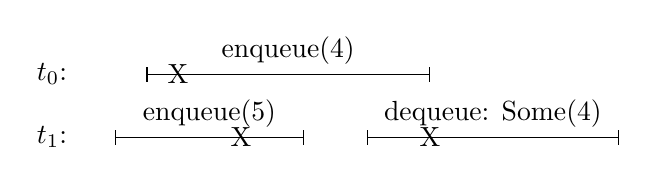
\begin{tikzpicture}[scale=0.8]
\draw (0,0) node {$t_0$:}; 
\draw[|-|] (1.5,0) -- node[above] {\scalashape enqueue(4)} (6,0);
\draw(2,0) node{X};
\draw (0,-1) node {$t_1$:}; 
\draw[|-|] (1,-1) -- node[above] {\scalashape enqueue(5)} (4,-1);
\draw(3,-1) node{X};
\draw[|-|] (5,-1) -- node[above] {\scalashape dequeue: Some(4)} (9,-1);
\draw(6,-1) node{X};
\end{tikzpicture}


Note that the history
\begin{scala}
  enqueue(4), enqueue(5), dequeue: Some(4)
\end{scala}
would be valid on a corresponding sequential queue. 
\end{slide}

%%%%%

\begin{slide}
\heading{Linearization examples}

But with different linearization points, a dequeue of 5 might have happened.

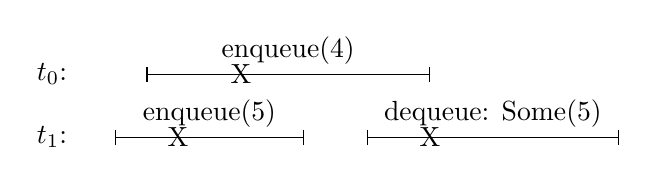
\begin{tikzpicture}[scale=0.8]
\draw (0,0) node {$t_0$:}; 
\draw[|-|] (1.5,0) -- node[above] {\scalashape enqueue(4)} (6,0);
\draw(3,0) node{X};
\draw (0,-1) node {$t_1$:}; 
\draw[|-|] (1,-1) -- node[above] {\scalashape enqueue(5)} (4,-1);
\draw(2,-1) node{X};
\draw[|-|] (5,-1) -- node[above] {\scalashape dequeue: Some(5)} (9,-1);
\draw(6,-1) node{X};
\end{tikzpicture}

Again note that the history
\begin{scala}
  enqueue(5), enqueue(4), dequeue: Some(5)
\end{scala}
would be valid on a corresponding sequential queue. 
\end{slide}

%%%%%

\begin{slide}
\heading{Linearization examples}

With the following timeline, the dequeue must return 5: any other return would
not be linearizable.
%
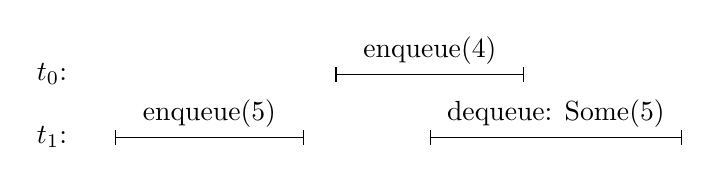
\begin{tikzpicture}[scale=0.8]
\draw (0,0) node {$t_0$:}; 
\draw[|-|] (4.5,0) -- node[above] {\scalashape enqueue(4)} (7.5,0);
%\draw(3,0) node{X};
\draw (0,-1) node {$t_1$:}; 
\draw[|-|] (1,-1) -- node[above] {\scalashape enqueue(5)} (4,-1);
%\draw(2,-1) node{X};
\draw[|-|] (6,-1) -- node[above] {\scalashape dequeue: Some(5)} (10,-1);
%\draw(6,-1) node{X};
\end{tikzpicture}

And the following history is not linearizable, because the queue is non-empty
throughout $t_2$'s operation.
%
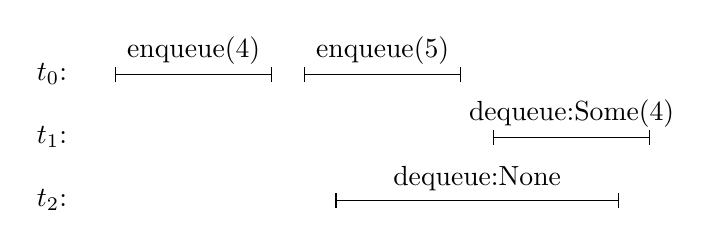
\begin{tikzpicture}[scale=0.8]
\draw (0,0) node {$t_0$:}; 
\draw[|-|] (1,0) -- node[above] {\scalashape enqueue(4)} (3.5,0);
\draw[|-|] (4,0) -- node[above] {\scalashape enqueue(5)} (6.5,0);
\draw (0,-1) node{$t_1$:};
\draw[|-|] (7,-1) -- node[above] {\scalashape dequeue:Some(4)} (9.5,-1);
\draw (0,-2) node{$t_2$:};
\draw[|-|] (4.5,-2) -- node[above] {\scalashape dequeue:None} (9,-2);
\end{tikzpicture}
\scalaMid
\end{slide}

%%%%%


%%%%%

\begin{slide}
\heading{Synchronous channels}

It is important that we use \emph{synchronous channels} in the server-based
queue.  Suppose we used buffered channels.  Then the following behaviour is
possible.
%
\begin{enumerate}
\item Thread $t_1$ calls |enqueue(5)|, but the value~|5| stays in the
  |enqueueChan|, even after $t_1$ returns;

\item Thread $t_2$ calls |dequeue|, and the server sends it |None|.
\end{enumerate}

Alternatively
%
\begin{enumerate}
\item The server sends |None| on |dequeueChan|, and that value stays in the
  channel; 

\item Thread $t_1$ calls |enqueue(5)|, and this value is received and stored
  by the server; 

\item Thread $t_2$ calls |dequeue|, and receives the |None| sent earlier.
\end{enumerate}
\end{slide}

%%%%%

\begin{slide}
\heading{Synchronous channels}

Using synchronous channels, the invocations have an effect in the order of the
channel communications.  This order is compatible with the order of the
invocations calls and returns.

We will always use synchronous channels when implementing a concurrent
datatype using a server process.   
\end{slide}


%%%%%

\begin{slide}
\heading{Testing for linearizability}

How can we test for linearizability?

Basic idea: 
%
\begin{itemize}
\item Run some threads on the concurrent queue, performing random |enqueue|
and |dequeue| operations, and record the history of operation calls and
returns;

\item Search for a corresponding sequential history that explains
linearizability, and that is a valid history for the corresponding sequential
datatype.  If none is found, signal an error.
\end{itemize}
%
Repeat many times.
\end{slide}

%%%%%

\begin{slide}
\heading{Testing for linearizability}

I've developed a framework to support such testing\footnote{{Testing
    for Linearizability}, Gavin Lowe, \textit{Concurrency and Computation},
    Practice and Experience, 29 (4), 2017,
  \url{http://www.cs.ox.ac.uk/people/gavin.lowe/LinearizabiltyTesting/}.},
and, in particular, investigated algorithms for testing whether a concurrent
history is linearizable.

In the next slides, we'll see a stripped-down testing script that uses this
(the full version can be used with multiple concurrent queue implementations,
and replaces the numerical constants by variables, specifiable via the command
line).

\vfill
\end{slide}

%%%%%

\begin{slide}
\heading{A small testing script}

The test program works on a concurrent datatype of some type~|C|; here we use
a |TotalQueue| containing |Int|s.  The test program
also requires a corresponding, \emph{immutable, deterministic}
sequential specification datatype~|S|, here an immutable queue from the Scala
API.
%
\begin{scala}
object QueueTest{
  type C = TotalQueue[Int]
  type S = scala.collection.immutable.Queue[Int]
  ...
}
\end{scala}
\end{slide}

%%%%%

\begin{slide}
\heading{A small testing script}

For each operation |op : A| on the concurrent datatype, we need a
corresponding function |seqOp : S => (A, S)| on the sequential datatype, which
returns the same value as the concurrent operation\footnote{More precisely,
  the two values should be equal, as tested using the ``{\scalashape ==}''
  method.}, paired with the new value of the sequential datatype.  These are
normally simple wrappers around API code.
%
\begin{scala}
  def seqEnqueue(x: Int)(q: S) : (Unit, S) = ((), q.enqueue(x))
  def seqDequeue(q: S) : (Option[Int], S) =   
    if(q.isEmpty) (None, q) 
    else{ val (r,q1) = q.dequeue; (Some(r), q1) }
\end{scala}
\vfill
\end{slide}

%%%%%

\begin{slide}
\heading{A small testing script}

The main part of the test program is the definition of a |worker| function
that performs and logs operations on the concurrent datatype, associating each
concurrent operation with a corresponding operation on the sequential
datatype.  Here, the worker performs 200 operations; each is (with probability
0.3) an enqueue of a random value, or (with probability~0.7) a dequeue.
\begin{scala}
  def worker(me: Int, log: LinearizabilityLog[S, C]) = {
    val random = new scala.util.Random
    for(i <- 0 until 200)
      if(random.nextFloat <= 0.3){
        val x = random.nextInt(20)
        log(_.enqueue(x), s"enqueue($x)", seqEnqueue(x))
      }
      else log(_.dequeue, "dequeue", seqDequeue)
  }
\end{scala}
\end{slide}

%%%%%

\begin{slide}
\heading{A small testing script}

The worker takes a log object |log| as a parameter; each operation is
performed and logged via a call to |log|, taking three parameters:
%
\begin{itemize}
% \item
% The identity of the thread doing the operation;

\item
The operation to be performed on the concurrent datatype;

\item A string describing the operation (this is used in debugging output in
the case that a non-linearizable history is found, and is also used internally
for optimisations; semantically different operations should have different
strings);

\item
The corresponding operation on the sequential datatype.
\end{itemize}

The call to |log| logs the invocation of the concurrent operation,
performs the concurrent operation, and logs the result returned.
\end{slide}
\begin{slide}
\heading{A small testing script}

The main test for linearizability is performed at line~\ref{line:maintest},
below, repeated so as to consider 1000 histories.  The  tester
takes as arguments: the sequential datatype; the concurrent datatype; the
number |p| of worker threads to run; and the definition of a worker thread.
%
\begin{scala}[numbers=left,numberstyle=\scriptsize]
  def main(args: Array[String]) = for(i <- 0 until 1000){
    val concQueue = new ServerTotalQueue[Int] // The concurrent queue
    val seqQueue = Queue[Int]() // The sequential specification queue
    val tester = LinearizabilityTester[S, C](seqQueue, concQueue, 4, worker _)
    assert(tester() > 0)£\label{line:maintest}£
  }
\end{scala}
%
The linearizability tester runs |p| workers concurrently, logging the
operation calls on the concurrent datatype.  It then tests whether the
resulting history is linearizable, returning a positive result if so.
\end{slide}

%%%%%

\begin{slide}
\heading{Controlling the search space}

The algorithm for testing linearizabilty, in effect, considers all possible
linearizations of the history, i.e.~all ways of ordering the operations
consistent with the history.  It then tests whether that ordering is
compatible with the sequential datatype, i.e.~whether performing the
corresponding sequential operations in the same order would give the same
results. 

Thus the algorithm considers all  states that the sequential
specification object could get into after a prefix of such linearizations.
%
If there are too many such states, this will take a long time.  It's therefore
a good idea to design the test so that such bad cases are very unlikely.
\end{slide}

%%%%%

\begin{slide}
\heading{Controlling the search space}

With a queue, the linearizability tester considers all possible states of the
sequential queue formed by permuting concurrent enqueue operations.  This
number grows exponentially with the length of the queue.  We therefore try to
avoid the length of the queue growing too much.  We did this in the earlier
testing harness by making dequeues more frequent than enqueues.
\end{slide}

%%%%%

\begin{slide}
\heading{Logging}

By default, the linearizability tester logs operation calls and returns using
thread-local logs, pairing each event with a timestamp.  We saw a similar
technique in an earlier chapter.  If you're using an operating system that
doesn't support timestamps property, setting the optional parameter |tsLog| to
|false| will use a different type of log.
%
\begin{scala}
  val tester = LinearizabilityTester[S, C](
    seqQueue, concQueue, 4, worker _, £\scalastyle\color{red} tsLog = false£)
\end{scala}
\end{slide}

%%%%%

%% \begin{slide}
%% \heading{Exercise}

%% Implement and test a total concurrent stack using similar techniques.
%% \end{slide}
 % concurrent total queue, using a server
%\input{client-server4} % layering; conclusions

%%%%%

\begin{slide}
\heading{Summary}

\begin{itemize}
\item
Clients and servers; 

\item
Requests and responses;

\item
Different styles of reply channels;

\item
Testing via logging;

\item Queueing pending requests; blocking pending requests;

\item
Asynchrony; 

\item
Multiple channels or multiple types of request.
\end{itemize}

\end{slide}

\end{document}
